\documentclass[10pt]{beamer}

\usetheme[progressbar=frametitle]{metropolis}
\usepackage{appendixnumberbeamer}

\usepackage{booktabs}
\usepackage[scale=2]{ccicons}

\usepackage{pgfplots}
\usepgfplotslibrary{dateplot}

\usepackage{xspace}
\newcommand{\themename}{\textbf{\textsc{metropolis}}\xspace}

\title{Semantic Analysis in Rust}
\subtitle{Compiler Construction presentation}
\date{}
\author{Oussama Danba}

\begin{document}

\maketitle

\begin{frame}{Table of Contents}
  \setbeamertemplate{section in toc}[sections numbered]
  \tableofcontents[hideallsubsections]
\end{frame}

\section{General Information}
\begin{frame}{Monomorphic Type Checking}
    \begin{itemize}
        \item Wanted to do polymorphic type checking but settled for a robust monomorphic implementation.
        \begin{itemize}
            \item Exception for print and isEmpty functions. Since the compiler generates these we don't have to check the function body!
        \end{itemize}
        \item Binding time analysis, type checking, and overloading is all done in one pass. In total about 400 lines of code.
        \begin{itemize}
            \item First: Function headers are checked and added into the type environment
            \item Second: Global variables are checked and added into the type environment
            \item Third: Function bodies are checked
        \end{itemize}
    \end{itemize}
\end{frame}

\begin{frame}{Changing the AST}
    \begin{itemize}
        \item AST parsed so far parses more than the monomorphic type checking allows. Change the parser and AST accordingly.
    \end{itemize}
    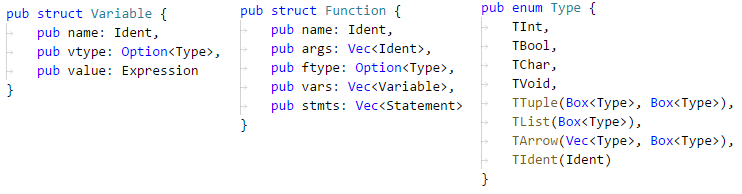
\includegraphics[width=\textwidth]{presentation2/AST.png}
\end{frame}

\begin{frame}{Changing the AST}
    \begin{itemize}
        \item AST parsed so far parses more than the monomorphic type checking allows. Change the parser and AST accordingly.
    \end{itemize}
    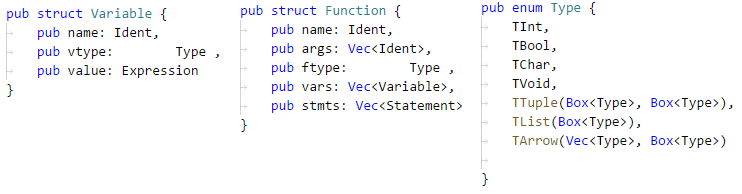
\includegraphics[width=\textwidth]{presentation2/AST-changed.png}
\end{frame}

% NOTE TO SELF: HIGHLIGHT THE ERRORS
\section{Type Environment}
\begin{frame}{Type Environment}
    \begin{itemize}
        \item Ideally a HashMap where the key is the identifier and the value a type.
            \begin{itemize}
                \item Since variables and functions can share identifiers we also need to store whether it is a variable or function (or use two separate type environments).
            \end{itemize}
        \item Whenever a variable a shadowed the original entry is kept since it may be needed later. (Multiple functions using a global variable for example)
    \end{itemize}
    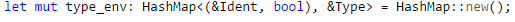
\includegraphics[width=\textwidth]{presentation2/type_env.png}
\end{frame}

\section{Analysing Expressions}
\begin{frame}{Expressions}
    Expressions can not introduce anything new into the type environment and all expressions return a type.
        \begin{itemize}
            \item We can thus write a function that analyses expressions and returns a type if the expression is well-formed!
        \end{itemize}
    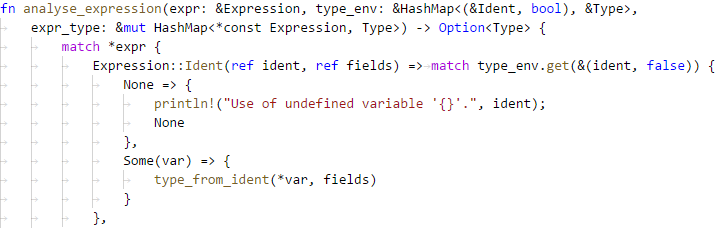
\includegraphics[width=\textwidth]{presentation2/expr_ident.png}
\end{frame}

\begin{frame}{Operator Overloading}
    Operators are expressions so we deal with operator overloading while dealing with expressions.
    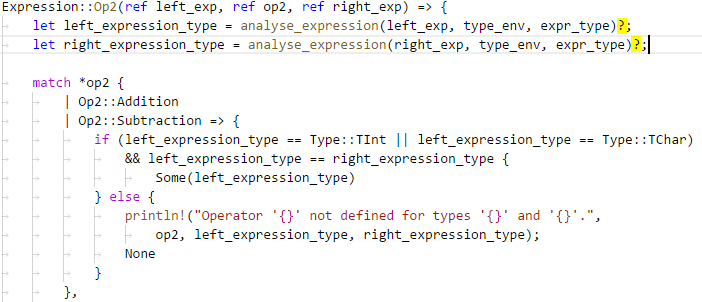
\includegraphics[width=\textwidth]{presentation2/expr_op2.png}
\end{frame}

\begin{frame}{Decorating the AST}
    During code generation we'd like to know the type of an expression (``return 1 : 2 : [];`` has what type?). During type checking we are certain what the type of an expression is so we might as well store it at this point so we don't have to check again during code generation.

    Thus a second environment called the expression environment is stored (omitted so far). The key is the address of the expression and the value is the type. No need to modify the AST.
    
    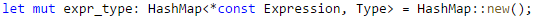
\includegraphics[width=\textwidth]{presentation2/expr_type.png}
\end{frame}

\begin{frame}{Decorating the AST}
    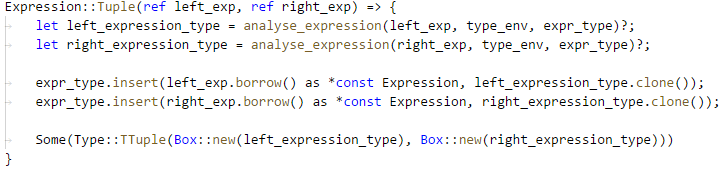
\includegraphics[width=\textwidth]{presentation2/expr_tuple.png}
\end{frame}
    
\section{Analysing Function Headers}
\begin{frame}{Analysing Function Headers}
    \begin{itemize}
        \item First: Check whether the function already exists in the type environment. Results in ``Function '\{\}' multiply defined.'' error.
        \item Second: Check whether amount of types match amount of declared variables. Results in appropriate error if not.
        \item Third: Enter function in type environment.
    \end{itemize}
\end{frame}

\section{Analysing Global Variables}
\begin{frame}{Analysing Global Variables}
    \begin{itemize}
        \item First: Check whether the variable if already defined and output error if so. Not strictly necessary but since global variables are allowed anywhere in-between functions shadowing might become ambiguous.
        \item Second: Analyse the expression at the right hand side. Early return if that fails.
        \item Third: Match specified type to the type of the expression. Output error if applicable.
        \item Fourth: Enter variable into type environment.
    \end{itemize}
    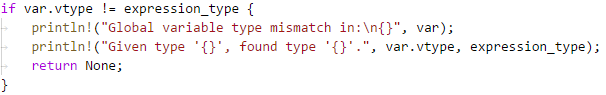
\includegraphics[width=\textwidth]{presentation2/global_var_mismatch.png}
\end{frame}

\section{Analysing Function Bodies}
\begin{frame}{Shadowing}
    First shadow the global variables with the function arguments. Then shadow the changed type environment with the variable declarations. (A global variable ``x'' may thus be shadowed by the function arguments and variable declarations!)

    Output applicable errors if anything goes wrong (for example a wrong variable declaration).
\end{frame}

\begin{frame}{Handling Statements}
    Handling statements is fairly straightforward. Types are checked whenever necessary (same for the existence of identifiers) and output errors if something fails. Any expression that is encountered is put into the expression environment. Returns are checked against the return type of the function.
    
    The largest difficulty is ensuring every path has a valid return value without introducing unnecessary returns. This is done by marking statements as having a guaranteed return.
\end{frame}

\begin{frame}{Handling Statements}
    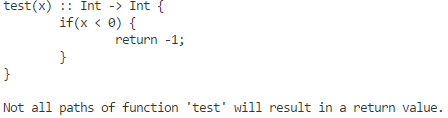
\includegraphics[width=\textwidth]{presentation2/test1.png}
\end{frame}

\begin{frame}{Handling Statements}
    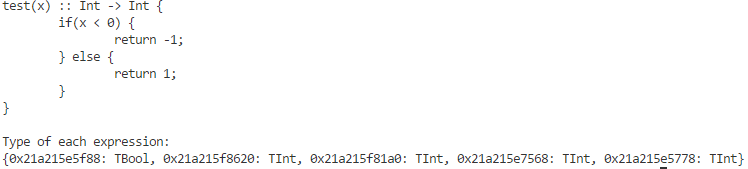
\includegraphics[width=\textwidth]{presentation2/test2.png}
\end{frame}

\begin{frame}{Handling Statements}
    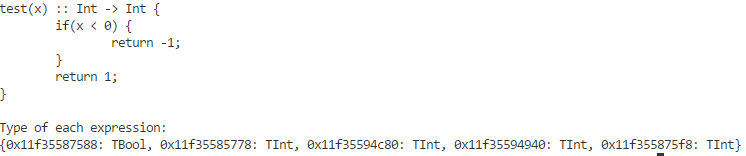
\includegraphics[width=\textwidth]{presentation2/test3.png}

    Note that for Void function there is an exception since there is an implicit return at the end.

    Also note that this can be nested as deep as wanted and it will keep working. An ``if-else'' statement will only guarantee a return if the bodies guarantee a return.
\end{frame}

\begin{frame}{Calling functions}
    Functions can call other functions. Obviously the given arguments have to match the function header stored! This is a small problem for isEmpty and print since we do not have polymorphic functions.
    
    Hardcoded exceptions for these. print will accept every type but will complain if more than one argument is given. isEmpty will accept every type as long as the outer type is a list (will also complain if more than one argument is given).
    
    We only have to check function headers as the bodies are generated based on the argument. Thus polymorphic print and isEmpty are emulated.
\end{frame}

\section{Some Examples}
\begin{frame}{Program that does not compile}
    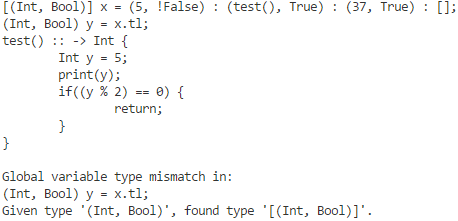
\includegraphics[width=\textwidth]{presentation2/test4.png}
\end{frame}

\begin{frame}{Program that still does not compile}
    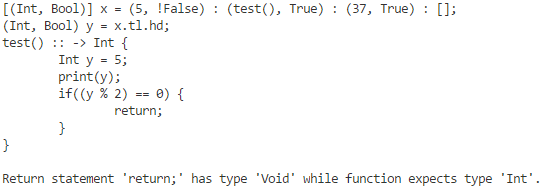
\includegraphics[width=\textwidth]{presentation2/test5.png}
    
    Let's make it recursive because we're writing something weird anyway.
\end{frame}

\begin{frame}{Program that \textit{still} does not compile}
    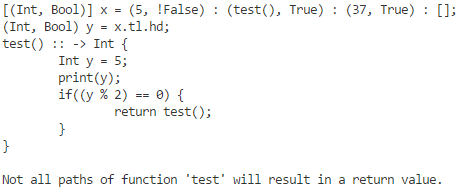
\includegraphics[width=\textwidth]{presentation2/test6.png}
\end{frame}

\begin{frame}{Program that compiles}
    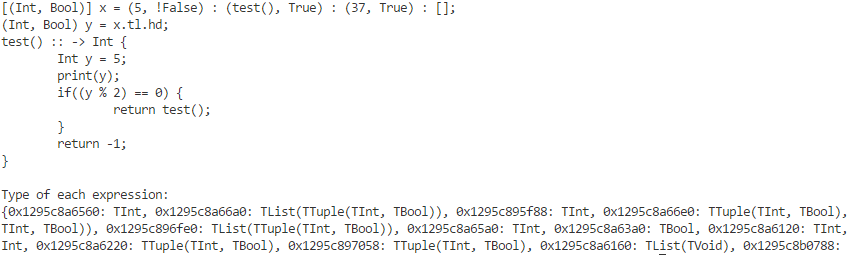
\includegraphics[width=\textwidth]{presentation2/test7.png}
\end{frame}

\section{Ending}
\begin{frame}{Current status}
    \begin{itemize}
        \item Semantic analysis is done and seems to pass all cases thrown at it (that should work)
        \item Reasonably happy with the code but the error handling could have been better by passing the error up (resulting in clearer return types)
        \item What to do about program entry point? Three ``obvious'' options:
        \begin{itemize}
            \item Mandate the existence of a main function
            \item Use the first function defined as entrypoint (probably a bad idea)
            \item Use a default entrypoint that does nothing (probably also a bad idea)
        \end{itemize}
    \end{itemize}
\end{frame}

{\setbeamercolor{palette primary}{fg=black, bg=yellow}
\begin{frame}[standout]
  Questions?
\end{frame}
}

\begin{frame}{License information}

  Get the source of this theme from

  \begin{center}\url{github.com/matze/mtheme}\end{center}

  The theme \emph{itself} is licensed under a
  \href{http://creativecommons.org/licenses/by-sa/4.0/}{Creative Commons
  Attribution-ShareAlike 4.0 International License}.

  \begin{center}\ccbysa\end{center}

\end{frame}

\end{document}
